	 \begin{htmlonly}
    
    
\usepackage{html, htmllist}
\usepackage{longtable}

\bodytext{bgcolor="#ffffff" link="#0033cc" vlink="#0033cc"}

%%%==================================================	
%%%==================================================	

% #1  mark defined by \label
% #2  a linktext 
% #3  a html link 
\newcommand{covlink}[3]{\htmladdnormallink{#2}{#3} \latex{(\ref{#1})} }


\newenvironment{covimg}[4]%
{
 \begin{figure}[htp]
  \begin{center}
   \latexonly
      \includegraphics[scale=#4]{#1/pict/#2}
   \endlatexonly  
   \html{\htmladdimg[align="center"]{pict/#2.png}}
   \caption{#3}
  \end{center}
 \end{figure} 
}{} 

\newenvironment{covimg2}[3]%
{ 
 \begin{figure}[htp]
  \begin{center}
     \latexonly
       \includegraphics[scale=#3]{#1/pict/#2}   
     \endlatexonly
     \html{\htmladdimg[align="center"]{pict/#2.png}}
  \end{center}
 \end{figure} 
}{}

\definecolor{output}{rgb}{0.,0.,1.}
\definecolor{depend}{rgb}{1.,0.65,0.}
\definecolor{required}{rgb}{0.58,0.,0.83}
\definecolor{optional}{rgb}{0.,0.39,0.}

\newcommand{\addimage}[1] {\html{\htmladdimg{pict/#1.png}}}

\newcommand{\addpict}[4] {\latexonly
	     \begin{figure}[!htbp]
			  \begin{center}
   	 		  \includegraphics[scale=#1]{#2}
   	 		  \caption{#3}
		 		  \label{#4}
			  \end{center}
	 		\end{figure}
	     \endlatexonly}



    \newcommand{\mapeditor}{\textbf{Map Editor}}
\newcommand{\covise}{\textbf{COVISE}}

    
    \end{htmlonly}

    \newcommand{\mymenubar}{\html{\htmlref{Menubar}{menubar}}\latex{{\bf Menubar} (section \ref{menubar})}}
    \newcommand{\mytoolbar}{\html{\htmlref{Toolbar}{toolbar}}\latex{{\bf Toolbar} (section \ref{toolbar})}} 
    \newcommand{\mycanvas}{\html{\htmlref{Visual Programming Area}{canvas}}\latex{{\bf Visual Programming Area} (section \ref{canvas})}} 
    \newcommand{\mydatabrowser}{\html{\htmlref{Data Object Browser}{data:viewer}}\latex{{\bf Data Object Browser} (section \ref{data:viewer})}} 
    \newcommand{\mydataviewer}{\html{\htmlref{Data Viewer}{data:viewer}}\latex{{\bf Data Viewer} (section \ref{data:viewer})}} 
    \newcommand{\mymodulebrowser}{\html{\htmlref{Module Browser}{modulebrowser}}\latex{{\bf Module Browser} (section \ref{modulebrowser})}} 
    \newcommand{\myicon}{\html{\htmlref{Module Icon}{icon}}\latex{{\bf Module Icon } (section \ref{icon})}} 
    \newcommand{\mycontrol}{\html{\htmlref{Control Panel}{control}}\latex{{\bf Control Panel} (section \ref{control})}} 
    \newcommand{\myparameter}{\html{\htmlref{Module Parameter}{parameter}}\latex{{\bf Module Parameter} (section \ref{parameter})}} 
    \newcommand{\mymessagearea}{\html{\htmlref{Message Area}{message}}\latex{{\bf Message Area} (section \ref{message})}} 
    \newcommand{\myactions}{\html{\htmlref{Module Actions}{actions}}\latex{{\bf Module Actions} (section \ref{actions})}} 
    \newcommand{\mychat}{\html{\htmlref{Chat Line}{chat}}\latex{{\bf Chat Line} (section \ref{chat})}} 
    \newcommand{\myworking}{\html{\htmlref{Working with Modules}{working}}\latex{{\bf Working with Modules} (section \ref{working})}} 
    \newcommand{\mysetting}{\html{\htmlref{Settings}{setting}}\latex{{\bf Settings} (section \ref{setting})}} 
    \newcommand{\mycolormap}{\html{\htmlref{Colormap Editor}{colormap}}\latex{{\bf Colormap Editor} (section \ref{colormap})}} 
    
    \newcommand{\trolltech}{\html{\htmladdnormallink{Trolltech }{http://www.trolltech.com}}\latex{{\bf Qt }(http://www.trolltech.com)}}
    \newcommand{\mycollab}{\html{\htmladdnormallink{distributed or collaborative }{../collab/collab.html}}}
  

    %----------------------------------------------------------------------------------------------------------------------------
    
    
    

	 \startdocument
	 \chapter{The Map Editor}
	 \label{qtmapeditor}

   
	 This chapter explains the usage of the {\covise} {\mapeditor}, how to work with modules, 
	 connect module ports to a map and modify module parameters. 
	 After reading this chapter you should be able to visualize your data within {\covise}. 

	 The graphical user interface is based on the {\bf Qt} software 
    from \trolltech. After typing \verb+covise+ on a command line or clicking on a covise icon the  
    {\mapeditor} top level window appears.
    
    \addimage{mapeditor}
	 \addpict{0.5}{mapeditor/pict/mapeditor}{\mapeditor containing a tutorial map}{figmapeditor}  
    
    The windows layout consists of the following main parts:

	 \begin{enumerate}
	    \item the \mymenubar
	    \item the \mytoolbar 
	    \item the \mycanvas which is used to show and edit a module network. 
	    \item the \mydatabrowser which contains a list of all available modules on a certain host sorted by categories.
	    \item the statusline which shows the number of existing messages from the {\bf Controller}, 
             modules and other {\covise} parts and the last content.
	    \item the \mychat which is only visible in collaborative working mode
	 \end{enumerate}
      
	


	 \section{Menubar}
	 \label{menubar}
	 
	 The {\bf Menubar} contains all items to 
	 \begin{itemize}
	 \item manage a {\covise} session,
	 \item execute dataflow networks (module maps),
	 \item work in collaborative or distributed mode \latex{( More details in chapter 5)},
	 \item get help information.
	 \end{itemize}

	 
    
    
	 
	 \subsection{File Menu}
    \label{fileMenu}

	 Most of the items in the {\it File} entry of the {\bf Menubar} are also avaible in the \mytoolbar: 

	 \addimage{menufile}
	 \addpict{0.5}{mapeditor/pict/menufile}{File Menu}{} 


	 \begin{itemize}
	 \item {\bf New} 
	 
	 allows you to generate new module networks from scratch. The whole canvas will be cleared,
	 also the parameters in the {\mycontrol} and all data objects are destroyed. 
	 Added hosts will remain in the session. 

	 \item {\bf Open...}  
	 
	 enables {\covise} to load a previously stored module network including the stored 
	 parameter settings. The current layout in the canvas is destroyed as if {\it New} would have been  
	 chosen. If modules are distributed and the used hosts have not yet been 
	 included in the session, the passwords for the participating hosts are required. 

	 The loaded network appears in the {\mycanvas}. Each module is represented by an icon. A \myicon 
	 consists of input data ports on the top, output data ports on the bottom, a label and a book icon.

	 \item {\bf Save} 

	 stores the current network and its parameters. This is possible at any time, even 
	 while working in collaborative mode. If a previously opened module network exists the same filename and 
    path is used for storing. Otherwise a file browser is opened.

	 \item {\bf Save As...} 

	 stores the current map and its parameters. A prompt appears asking for a storing location. 

	 \item {\bf Settings...} 

	 defines the layout and behaviour of the {\mapeditor}. The parameters are described in \mysetting.

	 \item {\bf Reset Layout} 

	 resets the default layout.

	 \item {\bf SnapShot} 

	 copies the content of the {\mycanvas} into a {\it png file}. If a network is open or has been previously saved 
    the current network is stored using this filename and path. Otherwise the current working directory is used.
	 
	 \item {\bf Quit}	

	 pops up an logout window \latex{(see Fig.\ref{figquitcovise})} when something was modified.
	 When \verb+Yes+ is selected the {\covise} session is closed. All participating processes on all attending 
    hosts are also terminated.

	 \addimage{quitcovise}
	 \addpict{0.5}{mapeditor/pict/quitcovise}{Quit COVISE}{figquitcovise}

	 \end{itemize}





	 \subsection{Execution Menu}
    \label{execmenu}

	 When executing a module network one module icon after the other shows a colored frame which
	 indicated that it operates. A module network can be executed once or repeatedly.

	 

	 \addimage{menuexec}
	 \addpict{0.5}{mapeditor/pict/menuexec}{Execution Menu}{figmenuexec}  

	 The settings are:

	 \begin{itemize}
	 \item {\bf Execute} 

	 the complete module network independent of the previous state. Stored parameter changes are applied.
	 This item is also avaible in the {\mytoolbar}.
    
	 Executing the module network beginning with a certain module is described in the 
    {\myactions}, {\myparameter} and {\mycontrol}. 

	 \item {\bf OnChange} 

	 behaves as an update. It initiates
	 an execution after every single parameter change. The  {\mycontrol} interactor {\it Player} and 
    {\it Sequencer} in play or reverse mode (not in single step) will automatically set {\it OnChange}
	 and start the execution of the map repeatedly until their ending condition
	 is met. You can also set {\it OnChange} explicitly within  the {\mycontrol}. 

	 \end{itemize}






	 \subsection{CSCW Menu}
	 \label{cscw}
         
	 \latex{More detailes about distributed and collaborative working mode can be foundin chapter 5.}
    \html{This menu entry contains items for a distributed or collaborative working mode}  
	 
	 Additional hosts can be introduced at nearly every time during a {\covise} 
	 session. It serves to use specific resources like supercomputers or fileservers. 
    The first three items of this menu entry are also available in the {\mytoolbar}.


	 \addimage{menucscw}
	 \addpict{0.5}{mapeditor/pict/menucscw}{Host Menu}{figmenuhost}  


	 \begin{itemize}
    
	 \item{\bf Request Master State}
       
	 A master/slave relationship is applied among participating partners of a 
	 session. This means, that at every point in time only one participant has 
	 control over the overall session, while the others can only watch ongoing 
	 actions performed by the master. All slave windows are insensitive for user 
	 input that influence the network consistency and parameters. Important events are spread 
    to all slaves. Therefore when a new 
	 network is generated or edited, every module icon and connection line between 
	 module ports also appears on the slave {\mapeditor} canvas. The modifications 
	 in the {\myparameter} and attached parameters in the {\mycontrol} are also 
	 spread to the slave sides. 
    
	 Clicking on the {\it RequestMasterState} item pops up an inquiry dialog on the master side, 
	 informing that a user on a slave host wants to become the master.

	 \addimage{masterrequest}
	 \addpict{0.5}{mapeditor/pict/masterrequest}{MasterRequest Window}{figmasterrequest}  

	 If the master rejects the action the requesting slave will be informed. 

	 %\addimage{requestdenied_}
	 %\addpict{0.5}{mapeditor/pict/requestdenied}{Deny of MasterRequest}{figrequestdenied} 

	 Otherwise the 
	 master/slave relationship between these two will be exchanged. As a result 
	 the greyed menus of the {\bf MapEditor} on the previously slave side are now in 
	 black, while all menu items on the previous master side except for the MasterRequest and the Help button
	  are now in grey. 

	 \item {\bf AddHost (Distributed Working)} 

	 This item adds another host to the current session.  No other {\mapeditor} or {\covise} session 
    will be started at that host. Only modules can be executed on this host.

	 \item {\bf AddPartner (Collaborative Working)} 

	 This item will invite a partner to participate in a current session. A  complete {\covise} session starts 
    on that host. The partner gets an own {\mapeditor}. The content of the local windows 
	 are duplicated to those windows. By default the invited partner is in a slave state, so he
	 can't initiate actions, until the master/slave relationship is changed via the item {\it Request Master State }.
	 All important events are spread to all slave user interfaces and 
	 all parameters and user actions are copied. The only enabled button in the {\mymenubar} of the partner 
	 is the {\it RequestMasterState} and the {\it Help} button.
    
    A host in the {\mymodulebrowser} can be deleted  by clicking on it with the right mouse button. This 
    action is not possible for the first host of a {\covise} session.
	 
	 Pressing {\it AddHost} or {\it AddPartner} will pop up the left 
    window \html{. Compare the below figure. } \latex{in Fig.\ref{fighost}. } In this window  
	 a existing can be selected or typed. The hostnames in the list are the same as in the 
	 scope {\it HostConfig} of the {\covise}  configuration file. When \verb+OK+ is pressed 
	 {\covise} will look for information about the requested host.
	 This is shown in the right window. 
	 The default values for the remote host are also taken from the scope {\it HostConfig} of the configuration file. 


    
    \addimage{addhost1} 
	 \addimage{addhost2}
 
	  \latexonly
	  \begin{figure}[!htbp]
	  \hspace{3cm}
	  \begin{minipage}[b]{.4\linewidth}
   	 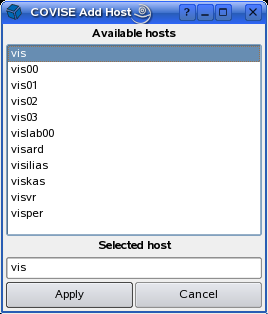
\includegraphics[scale=0.5]{mapeditor/pict/addhost1}
	  \end{minipage}
	  \hspace{1cm}
	  \begin{minipage}[b]{.4\linewidth}
   	 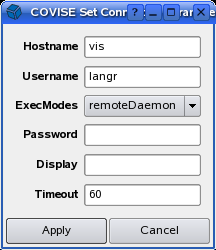
\includegraphics[scale=0.5]{mapeditor/pict/addhost2}
	  \end{minipage}
	  \caption{Adding hosts for distributed or dollaborative working mode}
	  \label{fighost}
	  \end{figure}
	  \endlatexonly

	 \end{itemize}

	 The timeout value specifies how many seconds a process will wait to be contacted by a new process
	 it initiated (e.g the Controller waiting for module). This parameter should be increased if the  network is slow.

	 The execeution mode specifies the command which should be used to start the {\bf CRB} 
	 on the remote computer. Possible execution modes are:

	 \begin{itemize}
	 \item {\bf rexec}

	 An userid and a password for the remote machine has to be typed. This is similar to login 
	 on a remote computer via telnet.

	 \item {\bf rsh}

	 In this case only the userid is required. A password on the remote machine is not needed. The rsh specific 
    rules for remote execution pf proceses have to be followed.

	 \item {\bf ssh}

	 Same as above, but a secure shell is needed. 

	 \item {\bf nqs}

	 This is not recommended. It can be used to put the {\bf CRB} into a batch queue.

	 \item {\bf manual} 

	 Manual means that someone has to start the {\bf CRB} process manually on the remote machine.
	 This can be useful for sessions across firewalls or access to the remote account is not available.
	 In this mode {\bf COVISE} writes a message in the window  \\
	 \verb/start "crb 31005 129.69.29.12 1005" on visper.hlrs.de/ . \\
	 The collaborativg partner has to type in this quoted string. 
    
	 \item {\bf remoteDamon} 

	 A remote {\bf COVISE} daemon has to run on the other machine. Currently this is only avalaible for Windows. 
    
	 \end{itemize}

	 When the remote host is successfully added, the remote username and hostname will appear 
    in the ist of hostnames of the {\mymodulebrowser} with a different color. 
 
 
 

	 \subsection{Module Menu}
    \label{modulemenu}
	 
	 Module icons in the {\mycanvas} can be manipulated.

	 \addimage{menumodule}
	 \addpict{0.5}{mapeditor/pict/menumodule}{Module Menu}{figmenuemodule}  

	 The settings are:

	 \begin{itemize}
	 \item {\bf Select all} 

	 All modules in the canvas are selected. Further operations can be applied on this group. 
    

	 \item {\bf Delete selected} 

	 Delete currently selected modules. 

	 \item {\bf Search modules...} 
    
    This entry opens a window which allows to enter a search string. All categories and/or modules containing 
    this string in the name will be highlighted. Icons of these module in the {\mycanvas} will also be highlighted.
	  
	 \addimage{search2}
	 \addpict{0.4}{mapeditor/pict/search2}{List of categories/modules after search operation}{figmenuesearch}  

	 \end{itemize}


   \clearpage
   

	 \subsection{Tools Menu}
    \label{toolmenu}

	 The items of this menu entry open additional window parts.
	 

	 \addimage{menutools}
	 \addpict{0.5}{mapeditor/pict/menutools}{Tools Menu}{figmenuexec}  

	 The settings are:

	 \begin{itemize}
	 \item {\bf Control Panel} 

	 Enables/disables an additional window on the right side. 
    
	 \addimage{mapeditor_with_cp}
	 \addpict{0.4}{mapeditor/pict/mapeditor_with_cp}{\mapeditor with Control Panel}{figmenumapcp}  
    
    \latex{More information about the {\bf Control Panel} is available in section \ref{control}.}
    \html{\htmlref{Control Panel}{control} shows more information.}
    

	 \item {\bf Data Viewer} 

	 Opens an additonal window containing the {\covise} {\mydataviewer} . 

	 \end{itemize}









	 \section{Available Help}
	 \label{help}


	 \subsection{Tooltips}
	 \label{tooltips}


	 A tooltip is a small piece of text that appears  when the cursor is hover a widget for a certain period of time.
    Tooltips are available for all icons of the {\mytoolbar}, the main buttons in the {\myparameter} window,   
	 the {\mycontrol}, the {\mysetting} and some other relevant items. 
    
    
	 \subsection{What's this ?}
	 \label{whatsthis}

    If more information is needed about a certain region of the {\mapeditor} the "What's This ?" mode is ideal. 
    The mode can be entered when the ? icon in the  {\mytoolbar} is clicked. The cursor changes to *** . Click a region 
    to obtain more information.
    
    
    \subsection{Online help}
    
    {\covise} opens a seperate help window when the item "Help" in the menubar is pressed. 
    This window is also available with \verb:Shift+F1:.
     
	 \addimage{menuhelp}
	 \addpict{0.5}{mapeditor/pict/menuhelp}{Available help items in the menubar}{figmenuhelp2_} 

	 The following help topics are available.

	 \begin{itemize}
	 \item {\bf Version} 
	 shows the version of your {\covise} installation. 
    
    \item {\bf Tutorial}
	 opens the online version of the Tutorial 

  	 \item {\bf User Guide} 
	 opens the online version of the User Guide

  	 \item {\bf Module Reference Guide} 
	 opens the online version of the Module Reference Guide
	 	 
	 \item {\bf Programming Guide} 
	 opens the online version of the Programming Guide 
	 
	 \end{itemize}





	 \section{Toolbar}
	 \label{toolbar}


	 The {\bf Toolbar} contains  
	 
	 \begin{enumerate}
	 \item icons for the most important actions
	 \item frequently used modules 
	 \end{enumerate}
	 
    
    
    
    
	 
	 \subsection{Toolbar Icons}

	 \addimage{toolicons} or   \addimage{toolbar2}
	 
    
	  \latexonly
	  \begin{figure}[!htbp]
	  \hspace{3cm}
	  \begin{minipage}[b]{.4\linewidth}
   	 
\includegraphics[scale=0.5]{mapeditor/pict/toolicons}
	  \end{minipage}
	  \hspace{1cm}
	  \begin{minipage}[b]{.4\linewidth}
   	 
\includegraphics[scale=0.5]{mapeditor/pict/toolbar2}
	  \end{minipage}
	  \caption{Available icons in the toolbar}
	  \label{figtoolicons}
	  \end{figure}
	  \endlatexonly
	  
	 These icons have the same behaviour as the items in the {\mymenubar}. The toolbar is dockable that means it can be 
    disconnect from the main window and show the content in an own separate window. A short decription
	 of the icons is given in the following list:

	 \begin{enumerate}
	 \item Load a new map into {\bf COVISE}
	 \item Save the current map. Overrides a given map name !!
	 \item Execute the module network 
	 \item The "What's This" help cursor 
	 \item Request the master state (only enabled if you are in slave mode) 
	 \end{enumerate}





    \subsection{Favourites}

    Favourites are often used modules. They can be used in the same manner as modules listed in the \mymodulebrowser.
	 
	 \addimage{favorites}
	 \addpict{0.5}{mapeditor/pict/favorites}{Frequently used modules}{figfavourites} 
    
    
	 \begin{enumerate}
	 \item The module name can be dragged into the {\mycanvas}. 
	 \item New favourite can be addeed to the list by dragging a module from the {\mymodulebrowser} to the favourite list. The drop 
    point marks the position in the list. 
	 \item A favourite can be removed from the list by dragging a favourite name to the {\mymodulebrowser} window. 
	 \item The list can be sorted by double clicking on a favourite name.
	 \end{enumerate}
	 

%\clearpage

	 \section{Module Browser}
	 \label{modulebrowser}

	 This area contains a hierarchy (tree) displaying the hostnames, category names and module names. When {\bf COVISE} is 
    started in single user mode only the name of the local host is shown in the tree. 
    
    \addimage{browser} 
	 \addpict{0.5}{mapeditor/pict/browser}{Parts of the Module Browser}{figbrowser} 
    
	 Modules running on a host appear in the same color as the host name in the list. The 
	 subdirectories of \verb+ ~/covise/ARCHSUFFIX/bin+ will be used as names of the categories. The files 
    in each category subdirectory are displayed as module names.  
    
    Short description of the category and the modules are shown as tooltips. Clicking on a 
    host with the right mouse button opens a popup menu with one single entry {\it Delete Host}. Clicking on this 
    item with the left mouse button will remove all modules running on that host and a possible 
    remote user interface. Clicking on a category or module with the right mouse button will open the {\bf COVISE} help system. 
    
    The modules shown for each category depend on the choosen modules in former sessions. To simplify the view 
    only modules which have been used before are shown. All other modules are hidden 
    behind the item {\it More..}. Clicking on this item will show all available modules in this category.
    
    The special category {\it All} contains all available modules in alphabetic order and the corresponding category.
   
	 \addimage{browser_all}
	 \addpict{0.5}{mapeditor/pict/browser_all}{The catgory ALL}{figbrowser1} 
    
    Interacting with the Module Browser is done in the following ways:
    
	 \begin{enumerate}
	 \item Clicking on the +/- sign open/close the corresponding category.
    \item Double clicking on a category name opens this specific category and closes all others.
    \item Clicking into the {\mycanvas} and typing / allows to enter a search string. All categories containing this string in the 
    module name will be highlighted. Icons of these module in the {\mycanvas} will also be highlighted.
	 \end{enumerate}
    
    
	 To start a module its module name has to be dragged to the canvas.  A {\myicon} on the canvas indicates, that the respective 
	 program representing the module has been started and waits for its execution. 


\clearpage
    
    
	 \section{Visual Programming Area (Canvas)}
	 \label{canvas}

	 This canvas is used to show the module network. Module icons,
	 that can be moves around, and connection lines between module ports can be seen. 
	 Executing a map visualizes the data using the {\bf Renderer} window. The execution of modules is indicated by 
	 highlighting the icon boundaries of currently executing modules. This red 
	 highlighting sweeps sequential through the processing pipeline.
    
	 \addimage{canvas}
	 \addpict{0.5}{mapeditor/pict/canvas}{The Visual Programming Area}{figcanvas} 



	 \subsection{Module Icon}
	 \label{icon}



	\latex{Fig. \ref{figicon}} \html{The above picture} shows a typically module icon. 
	 Each module is represented by such an icon. A module icon has 

	 \begin{itemize}
	 \item a background color which corresponds to the hostname color of the {\mymodulebrowser}.
    
	 \item input data ports
		 \begin{itemize}
		 \item {\bf pink}
       
       These ports have to be connected. Otherwise an error message appears.
		 \item {\bf green} 
       
       These ports can be optionally connected.
		 \end{itemize}
       
	 \item Output data ports
		 \begin{itemize}
		 \item {\bf blue}
       
       Normal output ports
		 \item {\bf orange}
       
       These output ports depend on an input port. If such an output port is selected 
		 the corresponding input ports change its color and become required. If disconnected the 
		 corresponding input port become green again.
		 \end{itemize}
       
	 \addimage{moduleicon}
	 \addpict{0.5}{mapeditor/pict/moduleicon}{Module Icon}{figicon} 
	 
	 \item a text label which consists of the module name and an instance number.
    
	 \item a book icon. If the closed book icon is selected, the {\myparameter} window of this module will be opened. 
		 In this window the module parameters are shown and can be changed. If an opened book icon is selected, the 
		 {\bf Module Parameter} window will be closed.
	 \end{itemize}



    \addimage{portinfo} 
	 \addpict{0.5}{mapeditor/pict/portinfo}{Available data types on a port}{figport1} 
    
    A tooltip shows port information like name, description and available datatypes.   
    If a data object exists (after the pipline has already been executed) information about the created
    data type are shown, otherwise the text {\it No data object} appears.



	 \subsection{Module Actions}
	 \label{actions}
    
	 A popup menu is shown, when the right mouse button is 
	 pressed on a module icon. This allows to 
	 perform the following module actions:  


	 \addimage{iconaction}
	 \addpict{0.5}{mapeditor/pict/iconaction}{Available Module Actions}{figiconaction} 


	 \begin{itemize}
	 \item {\bf Execute}

	 This executes the module network starting from the current module. It is typically 
	 more efficient to execute only a part of the map after having changed some parameters
	 instead of executing the whole network. I/O modules often need a lot of time to read in large
	 data files which is not necessary if a module parameter has been modified further 
	 down in the module chain.
	 
	 \item {\bf Delete} 

	 The module is deleted and disappears from the canvas. This function is also avaibale to remove a module group. 
	
	 \item {\bf Restart/Move} 
    
    Restarts the module with the current parameter values and connection lines.
    
    In distributed and collaborative working mode the module is moved to an other host 
    for execution. This means that the module is deleted on the current host and initialized 
	 on the other host. The current parameter and connections are moves too. This is only possible, 
	 if a further host was added.
	 
	 \item {\bf Clone/Copy} 

	 An exact copy of the module with the current parameter values is created. Connection lines 
    inside a copied module group are also picked.
    
    In distributed and collaborative working mode the module is copied to another host 
    for execution. This means that the module is initialized on the other host and remain on the original host. 
	 This is only possible, if an  additional host was added.
			
	 \item {\bf Rename}

	 The module is renamed. A new name is prompted for. This action is also avilable to add a label to a module group.
	 
	 \item {\bf Parameters} 

	 The \myparameter window is opened. This action has the same effect as clicking on a module book icon.

	 \item {\bf Help}

	 A HTML module description is shown in the Qt Help viewer, that is part of the {\mapeditor}. 

	 \end{itemize}





	 \subsection{How to move a module}

	 Hold down the left mouse button on the module icon.  The mouse pointer changes and you can move
	 the icon to a new position. The icon will follow the mouse pointer. Then release the mouse button. 
	 If the icons have connection lines to other ports, these lines will be repositioned too. 




	 \subsection{How to group modules}

	 \addimage{selectednodes}
	 \addpict{0.5}{mapeditor/pict/selectednodes}{Grouped module icons}{figselectednodes} 

	 YThere are two methods for grouping module icons on the canvas:

		 \begin{enumerate}
		 \item {\bf Specific Selection}

		 Press the SHIFT-Key and click on a module icon. The icon background changes to 
       the \html{\htmlref{user selected }{setting}} highlight color \latex{(see section \ref{setting})}. 
       Doing the same action on an already selected module icon deselects it.

		 \item {\bf Selection via a rubberband}

		 Click on an empty part of the canvas to determine the startpoint of the 
		 rubberband rectangle. Keep the mouse button pressed and move the mouse 
		 so that module icons which should be grouped together lie completely inside 
		 the rectangle. After the mouse button is released each of the icons inside the group
		 become red (the current hihglight color). Clicking on an empty part of the canvas ungroups the group. 
		 
       \item { \bf CTRL+A selects all modules on the canvas}.
		 \end{enumerate}


	


	 \subsection{Connecting Ports}
	 \label{connecting}

	 To build a module network you must connect the output ports of modules to the 
	 input ports of follow-on modules. Input and output ports of modules are 
	 color coded buttons according to the {\myicon}. A blue input 
	 port represents a data port, that has to be connected before a proper 
	 execution is possible. A green input port represents an optional port that can 
	 have a connection. Not all blue output ports need to be connected.  

    There are two methods for connecting ports:
    
    \begin{enumerate}
    \item{\bf Using the left mouse button}
    
	 The easiest way to establish proper connections without looking into 
	 the detailed descriptions of the module ports is by clicking with the left mouse 
	 button on the port of a module. This leads to  highlighting and/or blowing up of matching module ports, which 
    offer the appropriate data type. 
    
    \addimage{connect1} 
	 \addpict{0.4}{mapeditor/pict/connect1}{Generating a connection line: Image after clicking on a module port}{figiconaction} 
    
    Move the cursor to a heighlighted port. You now see a rubber line following 
    your mouse cursor. 
    
	 \addimage{connect2}
	 \addpict{0.4}{mapeditor/pict/connect2}{Generating a connection line: Move the cursor}{figiconaction2} 
    
    The connection is established when the mouse button is released within a port. 
    You can also directly click onto the the desired highlighted port. In the same 
	 way you have to connect all modules of a map.
    
	 \addimage{connect4}
	 \addpict{0.4}{mapeditor/pict/connect4}{Generating a connection line: Connection established}{figiconaction3} 


    \item{\bf Using the right mouse button}
    
	 Pressing/clicking on a port with the right mouse button pops up a menu that shows matching ports. 
    Selecting an item will create a connection line. This method is best when the network map has a lot a modules 
    some of them outside the visible range.
    
	 \addimage{connectright}
	 \addpict{0.4}{mapeditor/pict/connectright}{Generating a connection line with the right mouse button}{figiconaction4} 

    \end{enumerate}
    
    Move the mouse over a connection line. The line will be highlighted if the cursor is exactly on the 
    line. Delete the connection line by a double click or via a popupmenu that is shown 
    when using the right mouse button on a line.
    


	 %\clearpage

    
	 \section{Module Parameter}
	 \label{parameter}

	 Every module can present a detailed view of its input and output data objects 
	 as well as its parameters. Click with the left mouse button on the book icon of a module. 
    A new window appears on top of the {\bf MapEditor} window (default) or a new dockable widget becomes 
    visible inside the main {\mapeditor} window. The positions depends on your {\mysetting} parameter.

	 \addimage{moduleparameter1}
	 \addpict{0.5}{mapeditor/pict/moduleparameter1}{Module Parameter Window}{figmoduleparameter} 

	 Each parameter is represented  by 

	 \begin{itemize}
	 \item {\bf Name} 

	 This toggle button is used to map an interactor to 
	 the {\mycontrol} window. It contains also the name of the parameter. The type (
    {\it String, Boolean, Vector, Scalar, Slider, Choice, Browser}) and the description is shown as tooltip. 
    Most of the parameters were mapped with a standard appeareance that cannot be changed.

	 \item {\bf Appearance} 

	 Different appearance types for the parameter can be used {\it Scalar} and {\it Slider}. It is always
    possible to change the type.
     
    For the parameter type {\it Brower} and {\it Colormap} a folder icon is visible. Clicking on this icon 
    opens an additional browser window either below the parameter list inside the {\bf Module Parameter} window 
    or in a seperate window. Clicking on the open file icon will close the browser window.

	 \item{\bf Values} 

	 The value fields contain the parameter values. Depending on the parameter type different 
	 input fields to change the values are available. Values can be selectively overwritten . 
    The following list will show the different represenation of the parameter types

	 \begin{description}
	 \item[String] 
	 Just type in a string in a text input field.

	 \item[Boolean]
	 A toggle button is shown. Click on it to set/unset the state.
    
	 \item[Vector]
	 For each element of the vector a short text field is given which is used
	 as a string input field    

	 \item[Choice]
	 A combo box with the current item is shown. Click on the arrow to see all items.

	 \item[Scalar]
	 There are integer and float scalar parameters available. In the parameter window both are handled 
    in the same way. There are a text input field for the current value and one for a delta value. 
    The last value is only estimated. Please adapt this value. It is used by the interactors 
    to calculate a new current value.

	 \item[Slider]
	 Slider parameters are values that have a minimum and a maximum value, to be used to step up and down 
	 endless as a scalar parameter. They also have a delta value assigned that is used by the interactors.    
        
	 \item[Browser]
	 To choose a filename together with the proper path use either a string input field or 
	 a filebrowser. The first alternative is useful if the path and the 
	 filename is already known, otherwise open the file browser to find the file.	
    Depending on the settings the file browser 
    is opened in a seperate top level window or inside the {\bf Module Parameter} window.  
    
	 \addimage{filebrowser_in}
	 \addpict{0.4}{mapeditor/pict/filebrowser_in}{File Browser inside the Module Parameter window}{}
        
	 \item[Colormap]
	 How to modify a colormap is explained in {\mycolormap}.

    
	 \end{description}
	 \end{itemize}

   \clearpage
   
    
	 \section{Control Panel}
	 \label{control}

	 The purpose of the {\bf Control Panel} is the collection of graphical interactors which typically represent 
	 often used and changed parameters. 

    
	 \addimage{controlpanel1}
	 \addpict{0.5}{mapeditor/pict/controlpanel1}{Control Panel Window}{figcontrol}
	

	 Widgets corresponding to the parameter types are used for the layout of interactor. Interactors in the {\bf ControlPanel}  
	 allow the manipulation of parameters at every time without the need to 
	 pop up the {\myparameter}. By clicking the toggle button in the 
	 {\bf Module Parameter} window an interactor is generated. Its representation then appears in the 
	 {\bf Control Panel}.  

	 Changes made via interactors in the {\mycontrol} are updated in the 
	 corresponding parameter value fields of the {\myparameter} window.  This works also vice versa. 

	 Available interactors for each parameter are shown in the following list.

	 \begin{itemize}
	 \item {\bf String}
	 Only one string interactor is available. Just type in a string in a text input field.

	 \item {\bf Boolean}
	 A boolean interactor is realized as a toggle button. Click on it to set/unset the state.
	 This is the only one.

	 \item {\bf Vector}
	 A vector interactor has the same text input fields as in the {\myparameter} window. This is the default.	

	 \item  {\bf Choice}
	 As in the {\myparameter} window you see a combo box.  

	 \item {\bf Scalar}

	 \begin{itemize}
    
 			\item {\bf Scalar interactor = default}	This interactor has the same input fields as in the
			{\bf Module Parameter} window.

 			\item {\bf Sequencer interactor}	 Use this interactor like the control element of a
			videoplayer. There are no limits for the upper and lower value.
         
	 \end{itemize}	
    
	 \item {\bf Slider}
    
	 \begin{itemize}
 			\item {\bf Slider interactor = default}	

 			\item {\bf Player interactor}	Use this interactor like the control elements of a
			videoplayer. Keep in mind that the value has a range.		
         
	 \end{itemize}		
		
	 \item  {\bf Colormap}
	 This interactor works the same way as in the {\myparameter} window. Open/close a 
	 filebrowser if necessary.

	 \item  {\bf Browser}
	 This interactor works the same way as in the {\myparameter} window. Ppen/close a 
	 filebrowser if necessary.
     
	 \end{itemize}





	 \section{Data Objects, Data Viewer}
	 \label{data:viewer}

	 Data objects are created when a map is executed. The names of the data 
	 objects are generated generically, after the map was executed once. After a 
	 new execution the list is updated with the new names. 
    
    If you select a data object in the {\bf Data Object Browser}  more information is shown in the {\mydataviewer}
    on the right side of the {\mapeditor} 

	 \addimage{dataviewer}
	 \addpict{0.5}{mapeditor/pict/dataviewer}{Explore a COVISE Data Objects}{figdataviewer}
	 

	 Be careful if the data field is large or the data is located on another host, 
	 because this action will be time consuming.  

%\clearpage

	 \section{Colormap Editor}
    \label{colormap}

	 \addimage{colormap}
	 \addpict{0.5}{mapeditor/pict/colormap}{The Colormap Editor}{figcolormap}

         The purpose of the colormap editor is to define the ``transfer
         function'', i.~e.\ the mapping from scalar values to opacity
         (i.~e.\ inverse transparency) and colour values.
         The range of your data is mapped to $[0, 1]$ for the purpose of
         defining colour mappings.

         The transfer function is given as a piecewise linear mapping,
         the small triangles (``interpolation markers'') below the coloured bar
         in the picture above serve as nodes for linear interpolation.
         By clicking on an interpolation marker you can select it for
         manipulation:
         \begin{itemize}
         \item change its position by dragging it or by entering a new
         value in the input field labelled ``Current'', 
         \item modify colour and opacity -- this is described in
         more detail below.
         \end{itemize}

         The opacity can be modified by the self-named slider and input
         fields.
         For changing the colour values, there are more possibilities:
         \begin{itemize}
         \item enter red/green/blue values (in the range from $0$ to
               $1$) in the corresponding input fields,
         \item modify the colour according to the
         hue/saturation/value space: choose a colour hue and saturation in the large square
         and select the value in the coloured slider to the left of the
         large rectangular region, where the current colour is displayed,
         \item specify numerically hue, saturation and value in the
         corresponding input fields.
         \end{itemize}
         The resulting colour map is displayed in the large bar near the
         bottom.

         For speeding up, chose from predefined
         colour maps available in the configuration file with the
         ``Available Colormaps'' combo box, use the button labelled
         ``Save in ConfigFile'' for adding such a colour map.


%\clearpage
	
	 \section{Settings}
    \label{setting}

	 \addimage{settings}
	 \addpict{0.5}{mapeditor/pict/settings}{Settings for the Map Editor}{figsetting}

   Settings are used for the appearance and behaviour of the {\mapeditor}. These parameters are stored in the 
   file {\it mapqt.xml} which resides in \verb+$HOME/.covise+ and in \verb+$APPDATA\covise+ respectively.
   
   \begin{itemize}
   
   \item{\bf QT style (default)}
   
   defines the Qt theme used for the layout. These themes can differ from one operating system 
   to the other. On Linux systems the default style is used.
   
   \item{\bf Expert Mode (off)}
   
   If set all modules in the {\mymodulebrowser} are always shown.
   
   \item{\bf Auto connect hosts (on)}
   
   Autoconnect hosts of a loaded network if this map contains additional hosts.
   
   \item{\bf Embedded Filebrowser (on)}
   
   Opens the filebrowser for this module parameter inside the {\myparameter} window.
   
   \item{\bf Embedded OpenSG Renderer (off)}
   
   Integrate the OpenSG renderer windows inside the {\mapeditor} as a tab on the right side. Currently not implemented.
   
   \item{\bf Restore window layout (on)}
   
   After quitting the {\mapeditor} all positions and sizes of all windows are stored and reopened again the next time. 
   
   \item{\bf Error dialog boxes (off)}
   
   Off - show errors in the {\mymessagearea}. \\
   On  - pops up a dialog error window.
   
   \item{\bf User configuration path (~/.covise) }
   
   Path for storing files.
   
   \item{\bf Module History Length (50)}
   
   Maximal numbesr of modules that will be stored.
   
   \item{\bf Autosave file name (autosavemap.net)}
   
   After a certain amount of time a map is automatically stored using the above name.
   
   \item{\bf Autosave interval (120)}
   
   After a certain amount of time (120 sec) a map is automatically stored.
   
   \item{\bf Highlight module ports (on)}
   
   When connecting ports in the {\mycanvas} highlight matching ports.
   
   \item{\bf Highlight color (red)}
   
   Color name (from rgb.txt) for highlighting ports, connection lines and module icons.
   
   \item{\bf Enlarge module ports (on)}
   
   When connecting ports in the {\mycanvas} blow up module ports for better visibility .
   
   \item{\bf Enlarged port size (15)}
   
   Hight of enlarged module ports in pixel.
   
   \item{\bf Axis aligned connections (off)}
   
   When moving module icons in the {\mycanvas} the move of corresponding connection lines were shown (time comsuming)
   
   
   \end{itemize}



	
	 \section{Message Area}
    \label{message}

	 \addimage{message}
	 \addpict{0.5}{mapeditor/pict/message}{Message Area}{figmessage}

	 This scrollable text output window shows messages with different colors
	 \begin{itemize}
	 \item Error message are colored red.
	 \item Warning message are colored blue.
	 \item Info message are colored green.
	 \item Informations and control output produced by the {\mapeditor} itself are black.
	 \end{itemize}
    
	 Messages are sent from modules during their execution, the {\bf Controller} and the 
    request broker {\bf CRB}.





	 \section{Chat Line}
    \label{chat}


	 This editable text field is used for sending information to other partners joining a {\bf COVISE}  
    session. As expected, the chat line is shown for two or more partners only.  
    
